\section{Approach}
\label{sec:approach}
\begin{figure*}[th]
	%\vspace{-10pt}
	\centering
	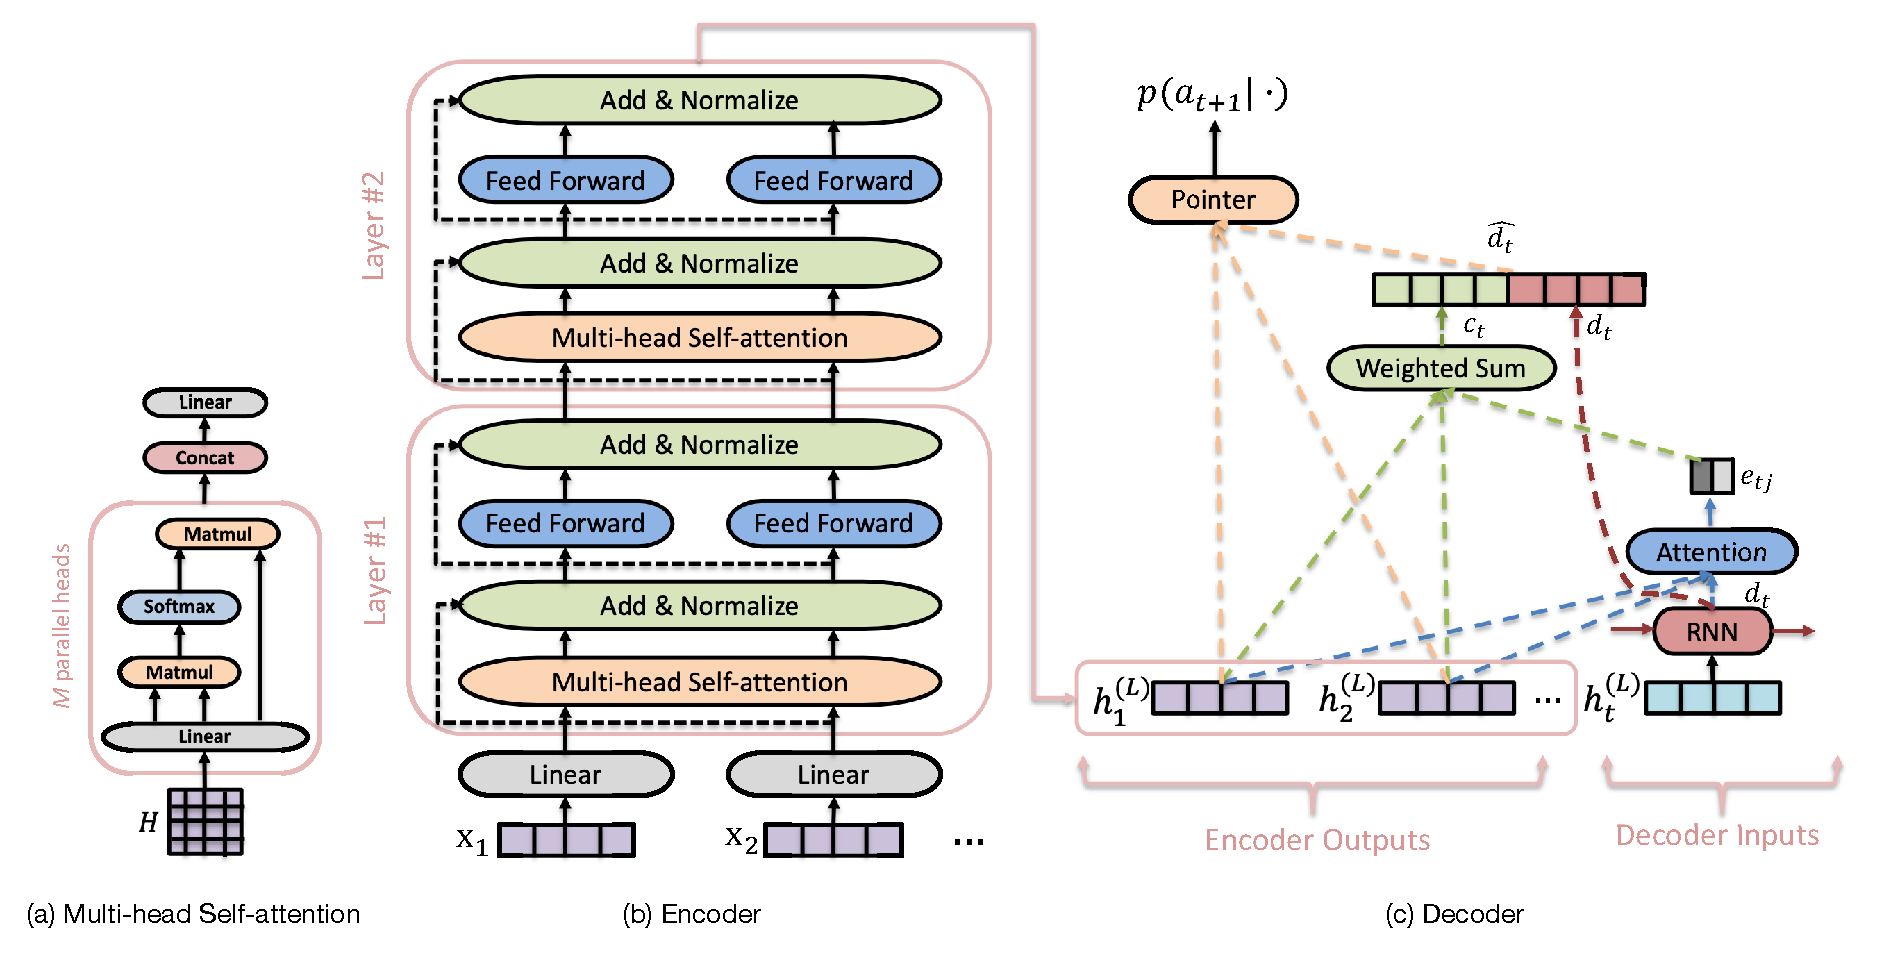
\epsfig{file=figures/transformer.eps, width=1.72\columnwidth}
	%\vspace{-10pt}
	\caption{The key modules of Graph Attention Networks (GAttN).}
		%, including (a) Multi-head Self-attention Layer, (b) Encoder Networks and (c) Decoder Networks.}
	\label{fig:transformer}
	%\vspace{-10pt}
\end{figure*}
In Sec. \ref{sec:problem_definition}, we formally define the exact-K recommendation problem based on searching for maximal scoring clique with $K$ nodes in a
specially constructed graph $\mathbb{G}(\mathcal{N},\mathcal{E})$ with $N$ nodes. 
The score of a clique is the overall probability of a user clicking or stratifying the corresponding card of $K$ items as in Eq. \ref{eq:objective}.
To tackle this specific problem, we first propose \emph{Graph Attention Networks} (GAttN) 
which follows the Encoder-Decoder Pointer framework \cite{vinyals2015pointer} with Attention mechanism \cite{vaswani2017attention,bahdanau2014neural}.
Then we adopt \emph{Reinforcement Learning from Demonstrations} (RLfD) which combines the advantages in behavior cloning \cite{torabi2018behavioral} and reinforcement learning \cite{sutton2000policy}, making it sufficient-and-efficient to train the networks.
%The remainder of this section provides details on our proposed approach.
 %For exact-K recommendation problem, node $i \in \{1,\dots, n\}$ in  graph $\mathbb{G}$ is represented by features $x_i$, e.g, the corresponding item id of the this node. In general, this model can be considered as a Graph Attention Network \cite{velickovic2017graph} and take graph structure into account by a masking the constraints. We define a clique (card) $A=\{a_i,\dots,a_K\}$ as a subset of permutations of the nodes, so $a_t \in \{i,..K\}$ and $a_t \neq a_{t_{'}} \forall t \neq t_{'}$. We solve this kind of maximal clique by a well-known encoder-decoder framework \cite{xxxx} and use a hybrid loss function to leverage advantages in reinforcement learning and supervise learning. We call this structure as the  Reinforce-supervised Graph Attention Networks. Moreover, scheduled sampling is introduced in supervised part to narrow the bias between training and testing whereas reinforcement learning adopts hill-climbing sampling to effectively avoid non-optimal local minimal and steadily increased reward throughout training. The remainder of this section provides details on how the proposed method works.
\subsection{Graph Attention Networks}
\label{sec:gattn}
The traditional encoder-decoder framework \cite{sutskever2014sequence} usually encodes an input sequence into a fixed vector by a recurrent neural networks (RNN)
and decodes a new output sequence from that vector using another RNN. 
For our exact-K recommendation problem, the encoder produces representations of all input nodes in graph $\mathbb{G}$, 
and the decoder selects a clique $A$ among input nodes by pointer, in which the constraint of clique is considered by masking.

\subsubsection{Input}
\label{sec:input}
%node $i \in \{1,\dots, n\}$ in  graph $\mathbb{G}$ is represented by features $x_i$, e.g, the corresponding item id of the this node.
We first define the input representation of each node in graph $\mathbb{G}(\mathcal{N},\mathcal{E})$.
Specifically in our problem, given candidate items set $S$ and user $u$,
we can represent the input $x_i$ of a node $n_i\in \mathcal{N}$ by combination of the features of corresponding item $s_i\in S$ and user $u$.
Here we use a simple fully connected neural network with nonlinear activation ReLU as:
\begin{small}
\begin{equation}
	x_i=ReLU(W_I[x_{s_i};x_u]+b_I),
\end{equation}
\end{small}
where $x_{s_i}$ and $x_u$ are feature vectors for item $s_i$ and user $u$ (e.g trainable embeddings of corresponding item and user IDs), $[a;b]$ represents the concatenation of vector $a$ and $b$, $W_I$ and $b_I$ are training parameters for input representation.

\subsubsection{Encoder}
\label{sec:encoder}
%\yu{1. The characteristic of our graph. So that we use multi-head self-attention to encode the graph.}
%\yu{2. What is multi-head self-attention? Its formulation and different from traditional Transformer model.}
%\yu{3. Give a figure and Equations.}
First of all, since the order of nodes in a undirected graph is meaningless,
the encoder network architecture should be permutation invariant,
i.e. any permutation of the inputs results in the same output representations. 
While the traditional encoder usually uses a RNN to convey sequential information, e.g., in text translation the relative position of words must be captured,
but it is not appropriate to our case.
Secondly, the representation for a node should consider the other nodes in graph, as there can exist some underlying structures in graph that nodes may influence between each other.
So it's helpful to represent a node with some attentions to other nodes.
As a result, we use a model like Self-attention,
it is a special case of attention mechanism that only requires a single sequence to compute its representation.
Self-attention has been successfully applied to many NLP tasks up to now \cite{yang2018query}, here we utilize it to encode the graph and produce nodes representations. 

Actually in this paper, the encoder that we use is similar
to the encoder used in Transformer architecture 
by \cite{vaswani2017attention} with multi-head self-attention.
Fig. \ref{fig:transformer}(b) depicts the computation graph of encoder.
From the $d_x$-dimensional input feature vector $x_i$ for node $n_i$, the encoder firstly computes initial $d_h$-dimensional graph node embedding (a.k.a representation) $h_i^{(0)}$ through a learned linear projection with parameters $W_E$ and $b_E$ as:
%\vspace{-10pt}
\begin{small}
\begin{equation}
	h_i^{(0)} = W_Ex_i + b_E.
\end{equation}
\end{small}
%\vspace{-10pt}
The node embeddings are then updated through $L$ self-attention layers, each consisting of two sub-layers:
a multi-head self-attention (MHSA) layer followed by a feed-forward (FF) layer.
We denote with $H^{(l)}=\{h^{(l)}_i\}_{1\leq i\leq N}$ the graph node embeddings produced by layer $l$,
and the final output graph node embeddings as $H^{(L)}$.
%are similar to the hidden state outputs of RNN encoder.

The basic component of MHSA is the scaled dot-product attention, which is a variant of dot-product (multiplicative) attention \cite{luong2015effective}.
%Compared with the standard additive attention mechanism \cite{bahdanau2014neural} which is implemented using a one layer feed-forward neural network, 
%the dot-product attention utilizes matrix production which allows faster computation.
Given a matrix of $N$ input $d$-dimensional embedding vectors $E\in \mathbb{R}^{N\times d}$,
the scaled dot-product attention computes the self-attention scores based on the following equation:
\begin{small}
\begin{equation}
\text{SelfAttention}(E)=softmax(\frac{EE^T}{\sqrt{d}})E,
\end{equation}
\end{small}
where $softmax$ is row-wise. 
More specifically,
MHSA sub-layers will employ $M$ attention heads to capture multiple attention information
and the results from each head are concatenated followed by a parameterized linear transformation to produce the sub-layer outputs.
Fig. \ref{fig:transformer}(a) shows the computation graph of MHSA.
Specifically in layer $l$, it will operate on the output embedding matrices
$H^{(l-1)}\in \mathbb{R}^{N\times d_h}$ from previous layer $l-1$
and produce the MHSA sub-layer outputs $\widehat{H^{(l)}}\in \mathbb{R}^{N\times d_h}$ as:
\begin{small}
\begin{equation}
\begin{aligned}
&\widehat{H^{(l)}}=[head_1;\dots;head_M]W_O, \\
\text{where}\ &head_i=\text{SelfAttention}(H^{(l-1)}W_{hi}),
\end{aligned}
\end{equation}
\end{small}
where $M$ is the number of heads,
$W_{hi}\in \mathbb{R}^{d_h\times d_k}$ is parameter for each head,
$W_O\in \mathbb{R}^{(Md_k)\times d_h}$ is parameter for linear transformation output,
and $d_k$ is the output dimension in each head.
%and computes a new $d_k$-dimensional embedding sequence $\hat{head_i}=\{\hat{h_{i1}},\dots,\hat{h_{iN}}\}$ of the same length. 
%The final results of a MHA sublayer at level $l$ is $h^{(l)}=\{\hat{h_i},\dots,\hat{h_n}\}$.
%Each MHA output element, $\hat{h_o}$, is concatenated from each attention head output:
%\begin{eqnarray}
%\hat{h_o} = [\hat{head_1};\dots;\hat{head_M}],\quad o\in\{1,\dots,N\}
%\end{eqnarray}
%Element of each attention head output $\hat{head_o}$, $\hat{h_{oi}}$ computed as weighted sum of a linearly transformed input elements: 
%\begin{eqnarray}
%\hat{h_{oi}}=\sum_{j=1}^{n}\alpha_{ij}(h_j^{l}W^V)
%\end{eqnarray}
%Each weight coefficient, $\alpha_{ij}$, is computed using a softmax function:
%\begin{eqnarray}
%\alpha_{ij}=\frac{\exp e_{ij}}{\sum_{k=1}^n\exp e_{ik}}
%\end{eqnarray}
%And $e_{ij}$ is computed using a compatibility function that compares two input elements:
%\begin{eqnarray}
%e_{ij}=\frac{1}{\sqrt{d_h}}(h_i^{l}W^{Q})(h_j^{l}W^{K})
%\end{eqnarray}
%Dot product was chosen for the compatibility function, which enables efficient computation. Linear transformations of the inputs add sufficient expressive power. 
%$W^Q, W^K, W^V\in R^{d_x*d_k}$ are parameter matrices. In this work, the MHA %sublayer uses $M = 8$ heads with dimensionality $d_k=\frac{d_h}{M} = 16$,
In addition to MHSA sub-layers, FF sub-layers consist of two linear transformations with a ReLU activation in between.
\begin{small}
\begin{equation}
h_i^{(l)} = W_{F2}ReLU(W_{F1}\widehat{h_i^{(l)}}+b_{F1})+b_{F2},
\end{equation}
\end{small}
where $W_{F1}, W_{F2}$ are parameter matrices, $\widehat{h_i^{(l)}}$ and $h_i^{(l)}$ represent embedding outputs of node $n_i$ in MHSA and FF sub-layers correspondingly.
We emphasize that those trainable parameters mentioned above are unique per layer.
Furthermore, each sub-layer adds a skip-connection \cite{he2016deep} and layer normalization \cite{ba2016layer}.

As a result, \emph{encoder} transforms $x_1,x_2,\cdots,x_N$ (original representations of nodes in graph) in Fig. \ref{fig:transformer}(b)
to $h_1^{(L)},h_2^{(L)},\cdots,h_N^{(L)}$ (embedding representations of these nodes, considering graph constructure information), which will be used in decoder in Fig. \ref{fig:transformer}(c).

\subsubsection{Decoder}
\label{sec:decoder}
%\yu{1. Why RNN decoder? The items in a card are related each other, we can use RNN to formulate. Specially LSTM for RNN.}
%\yu{2. Pointer with attention mechanism.}
%\yu{3. Beam search decode.}
%\yu{4. Give a figure and Equations.}
For exact-K recommendation problem, the output $A$ represents a clique (card) with $K$ nodes (items) in graph $\mathbb{G}$ that can be interrelated with each other.
Recently, RNN \cite{vinyals2015pointer} has been widely used to map the encoder embeddings to a correlated output sequence,
so does in our proposed framework. 
We call this RNN architecture decoder to decode the output nodes $A=\{a_1,\dots,a_K\}$.
Remember our goal is to optimize $P(A|S,u;\theta)$ defined in Sec. \ref{sec:problem_definition} (here we omit relevance score of $r=1$),
it is a joint probability and can be decomposed by the chain rule as follows:
%\vspace{-10pt}
\begin{small}
\begin{equation}
\label{eq:chain_rule}
\begin{aligned}
P(A|f(S,u;\theta)&=\prod_{i=1}^{K}p(a_i|a_1,\dots,a_{i-1},S,u;\theta)\\
&=\prod_{i=1}^{K}p(a_i|a_1,\dots,a_{i-1},f(S,u;\theta_e);\theta_d),
\end{aligned}
\end{equation}
\end{small}
where we represent encoder as $f(S,u;\theta_e)$ with trainable parameters $\theta_e$, and decoder trainable parameters as $\theta_d$.
The last term in above
Eq. \ref{eq:chain_rule} is estimated with RNN by introducing a state vector,
$d_i$, which is a function of the previous state $d_{i-1}$, and the previous output node $a_{i-1}$, i.e.
\begin{small}
\begin{equation}
p(a_i|a_1,\cdots,a_{i-1},f(S,u;\theta_e);\theta_d)=p(a_i|d_{i},f(S,u;\theta_e);\theta_d),
\end{equation}
\end{small}
where $d_i$ is computed as follows:
\begin{small}
\begin{eqnarray}
\label{eq:rnn_hidden}
d_i = 
\begin{cases}
g(0,0) & \text{if}\ i=1, \\
g(d_{i-1},a_{i-1}) & \text{otherwise},
\end{cases}
\end{eqnarray}
\end{small}
where $g(h,a)$ is usually a non-linear function (e.g. cell in LSTM \cite{hochreiter1997long} or GRU \cite{chung2014empirical}) that combines the previous state and previous output
(embedding of the corresponding node $a$ from encoder) in order to produce the current state.

Decoding happens sequentially, 
and at time-step $t \in \{1,\dots,K\}$, 
the decoder outputs the node $a_t$ based on the output embeddings from encoder
and already generated outputs $\{a_{t'}\}_{1\leq t'\leq t}$ which are embedded by RNN hidden state $d_t$. 
See Fig. \ref{fig:transformer}(c) for an illustration of the decoding process.
During decoding, 
$p(a_t|d_t,f(S,u;\theta_e);\theta_d)$ is implemented by an specific attention mechanism named \textbf{pointer} \cite{vinyals2015pointer},
in which it will attend to each node in the encoded graph 
and calculate the attention scores before applying \emph{softmax} function to get the probability distribution.
It allows the decoder to look at the whole input graph $\mathbb{G}(\mathcal{N},\mathcal{E})$ at any time
and select a member of the input nodes $\mathcal{N}$ as the final outputs $A$. 

For notation purposes, let us define decoder output hidden states as $(d_1,\dots,d_K)$,
the encoder output graph node embeddings as $(h_1^{(L)},\dots,h_N^{(L)})$.
At time-step $t$, decoder first glimpses \cite{vinyals2015order} the whole encoder outputs,
and then computes the representation of decoding up to now together with attention to the encoded graph, denoted as $\widehat{d_t}$ and the equation is as follows:
\begin{small}
\begin{eqnarray}
\label{eq:glimpse}
%\begin{aligned}
&e_{tj}=softmax(v_{D1}^T\tanh(W_{D1}d_t+W_{D2}h_j^{(L)})),j\in\{1,\dots,N\}, \nonumber\\
&c_t=\sum_{j=1}^{N}e_{tj}h_j^{(L)},\ \widehat{d_t}=[d_t;c_t],
%\end{aligned}
\end{eqnarray}
\end{small}
where $W_{D1}$, $W_{D2}$ and $v_{D1}$ are trainable parameters.
After getting the representation of decoder at time-step $t$,
we apply a specific attentive pointer with masking scheme to generate feasible clique from graph.
In our case, we use the following masking procedures: 
\begin{inparaenum}
\item nodes already decoded are not allowed to be pointed,
\item nodes will be masked if disobey the clique constraint rule among the decoded subgraph.
\end{inparaenum}
And we compute the attention values as follows:
%For the RNN, we use the state after the output gate has been component-wise multiplied by the cell activations. We compute the compatibility of the hidden states $d_t$ with all nodes and use $u_j^t$ as pointers to the input graph nodes. For faster training and generating feasible cards, we have used a masking scheme which sets the log-probabilities of infeasible cards to 1 or forces a card if a particular condition is satisfied. In our case, we  use the following masking procedures:(i) nodes which is already output are not allowed to be pointed; (ii) node will be masked if it obey the constraint rules among the decoded subgraph:
%\vspace{-10pt}
\begin{small}
\begin{equation}
\label{eq:pointer}
u_{tj}=
\begin{cases}
v_{D2}^T\tanh{(W_{D3}\widehat{d_t}+W_{D4}h_j^{(L)})},\ \ \text{otherwise},  \\
-\infty,\ \  \text{if node $n_j$ should be masked,}
%n_j\in \{a_{t'}\}_{1\leq t'\leq t} \| c_k(a_{t'},j) \neq 1 \quad \forall t' < t.
\end{cases} \\
%\vspace{-10pt}
\end{equation}
\end{small}
where $v_{D2}$, $W_{D3}$, and $W_{D4}$ are trainable parameters.
Then \emph{softmax} function is applied to get the pointing distribution towards input nodes, as follows:
%\vspace{-10pt}
\begin{small}
\begin{equation}
p(a_t|d_t,f(S,u;\theta_e);\theta_d)=softmax(u_{tj}),\ j\in\{1,\dots,N\}.
%\vspace{-10pt}
\end{equation}
\end{small}
We mention that the attention mechanism adopted in Eq. \ref{eq:glimpse} and \ref{eq:pointer} is following Bahdanau et al \cite{bahdanau2014neural}.
At the period of decoder inference, we apply technique of beam search \cite{vinyals2015show}.
%\yu{How to solve combinational information for card?}
It is proposed to expand the search space and try more combinations of nodes in a clique (a.k.a items for a card) to get a most optimal solution.

To summarize, \emph{decoder} receives embedding representations of nodes in graph $\mathbb{G}$ from encoder, and selects clique $A$ of $K$ nodes with attention mechanism.
With the help of RNN and beam search, decoder in our proposed GAttN framework is able to capture the combinational characteristics of the $K$ items in a card.

%Then, we compute output probabilities $p(a_t|X,A_{1:t-1})$ at each output time $t$ as follows:
%\begin{eqnarray}
%p(a_t|X,A_{1:t-1}) = softmax(u_j^t) \quad j\in(1,\dots,N)
%\end{eqnarray}
%where softmax normalizes the vector $u_t$ (of length $N$) to be the "attention" mask over the inputs graph node embeddings, and $v$, $W_{d1}$, and $W_{d2}$ are learnable parameters of the model. 

\subsection{Reinforcement Learning from Demonstrations}
\label{sec:rlfd}
\subsubsection{Overall}
%\yu{1. RL definition of our method.}
%\yu{2. What is RL from Demonstrations?}
%\yu{3. Why we use RL from Demonstrations?}
In our proposed GAttN framework,
we represent encoder as $f(S,u;\theta_e)$ which can be seen as \textbf{state} $\mathcal{S}$ in RL,
and we represent decoder as $P(A|f(S,u;\theta_e);\theta_d)=P(A|\mathcal{S};\theta_d)$ which can be seen as \textbf{policy} $\mathcal{P}$ in RL. 
%Here we omit relevance of $r=1$ in policy function.
%$P(A|f(S,u;\theta_e);\theta_d)$ is the joint probability of card of items and can be decomposed by the chain rule:
%\begin{equation}
%P(A|f(S,u;\theta_e);\theta_d) = \prod_{i=1}^{K}p(a_i|a_1,\dots,a_{i-1},f(S,u;\theta_e);\theta_d).
%\end{equation}
%Where $p(a_i|a_1,\dots,a_{i-1},f(S,u;\theta_e);\theta_d)$ is implemented by \textbf{pointer},
%in which it will attend to each node in the encoded graph and calculate the attention scores before applying \emph{softmax} function to get the probability distribution
%(refer to Section \ref{sec:decoder} for details).
A \emph{Reinforcement Learning from Demonstration} (RLfd) agent, possessing
both an objective reward signal and demonstrations, is able to
combine the best from both fields.
This framework is first proposed in domain of Robotics \cite{nair2018overcoming}.
Learning from demonstrations is much sample efficient and can speed up learning process,
leveraging demonstrations to
direct what would otherwise be uniform random exploration and
thus speed up learning. 
While the demonstration trajectories may be noisy or sub-optimal,
so policy supervised from such demonstrations will be worse too.
And learning from demonstrations is not directly targeting the objective which makes the policy fall into local-minimal.
%\yu{Weakness of Learning from Demonstration}.
%\yu{Strength of Reinforcement Learning.}
On the other hand,
training policy by reinforcement learning can directly optimize the objective reward signal,
witch allows such an agent to eventually outperform a
potentially sub-optimal demonstrator.

\subsubsection{Learning from Demonstrations}
\label{sec:supervise}
Learning from demonstrations can be seen as behavior cloning imitation learning \cite{torabi2018behavioral},
it applies supervised learning for policy (mapping states to actions)
using the demonstration trajectories as ground-truth.
We collect the ground truth clicked/satisfied cards $A^*=\{a_i^*\}_{1\leq i\leq K}$ given user $u$ and candidate items set $S$ as
demonstration trajectories and formulated as $P_{data}^{S}(A^*|S,u)$,
we can define the following loss function based on cross entropy $CrossEntropy$ of the generated cards $P(A|S,u;\theta)$ and demonstrated cards $P^S_{data}(A^*|S,u)$.
\begin{small}
\begin{equation}
\begin{aligned}
\mathcal{L}_{S}(\theta)&=\sum_{S,u}{CrossEntropy(P(A|S,u;\theta),P_{data}^{S}(A^*|S,u))} \\
&= -\sum_{S,u,A^*\in P_{data}^{S}}\log{P(A^*|S,u;\theta)} \\
%&= -\sum_{S,u,A^*\in P_{data}^{S}}\log{P(A^*|f(S,u;\theta_e);\theta_d)} \\
&= -\sum_{S,u,A^*\in P_{data}^{S}}\sum_{i=1}^{K}\log{p(a_i^*|a_1^*,\cdots,a_{i-1}^*,\mathcal{S};\theta_d)} \\
&= -\sum_{S,u,A^*\in P_{data}^{S}}\sum_{i=1}^{K}\log{p(a_i^*|d_i^*,\mathcal{S};\theta_d)},
\end{aligned}
\label{eq:cross_entropy}
\end{equation}
\end{small}
where $d_i^*$ in the last term is state vector estimated by a RNN defined in Eq. \ref{eq:rnn_hidden} with inputs of $d_{i-1}^*$ and $a_{i-1}^*$.
%and is computed here as follows:
%The last term in the above
%Equation \ref{eq:cross_entropy} is estimated by a recurrent neural network (RNN) with parameters $\theta_d$ by introducing a state vector,
%$h_i$, that is a function of the previous state, $h_{i-1}$, and the previous output item, $a_{i-1}^*$, i.e.
%\begin{equation}
%\log{p(a_i^*|a_1^*,\cdots,a_{i-1}^*,\mathcal{S};\theta_d)} =\log{p(a_i^*|h_{i},\mathcal{S};\theta_d)},
%\end{equation}
%where $h_i$ is computed by a recurrent neural network as follows:
%\begin{small}
%\begin{eqnarray}
%d_i^* = 
%\begin{cases}
%g(0,0) & \text{if}\ i=1, \\
%g(d_{i-1}^*,a_{i-1}^*) & \text{otherwise}.
%\end{cases}
%\end{eqnarray}
%\end{small}
%Where $g(h,a)$ is usually a non-linear function (e.g. cell in LSTM) that combines the previous state and the previous output
%(embedding from encoder of the corresponding item $a$) in order to produce the current state.
This means that the decoder model focuses on learning to output the next item of the card given the current state of the model
AND previous ground-truth items.

\paragraph{SUPERVISE with Policy-sampling.}
During inference the model can generate a full card $A$ given state $\mathcal{S}$ by generating one item at a time
%,and advancing time by one step
until we get $K$ items.
For this process, at time-step $t$, the model needs the output item $a_{t-1}$ from the last time-step as input in order to produce $a_t$.
Since we don't have access to the true previous item, we can instead either select the most likely one given our model or sample according to it.
In all these cases, if a wrong decision is taken at time-step $t-1$, the model can be in a part of the state space that is very different from those visited from the training distribution and for which it doesn't know what to do.
Worse, it can easily lead to cumulative bad decisions.
We call this problem as discrepancy between training and inference \cite{bengio2015scheduled}.
%Beam search \cite{vinyals2015show} can alleviate this problem to a certain degree but can't solve it in natural.

In our work, we propose \emph{SUPERVISE with Policy-sampling} to bridge the gap between training and inference of policy.
We change the training process from fully guided using the true previous item,
towards using the generated item from trained policy instead.
The loss function for \emph{Learning from Demonstrations} is now as follows:
\begin{small}
\begin{equation}
\label{eq:L_S}
\begin{aligned}
\mathcal{L}_{S}(\theta)&=-\sum_{S,u,A^*\in P_{data}^{S}}\sum_{i=1}^{K}\log{p(a_i^*|a_1,\cdots,a_{i-1},\mathcal{S};\theta_d)} \\
&=-\sum_{S,u,A^*\in P_{data}^{S}}\sum_{i=1}^{K}\log{p(a_i^*|d_{i},\mathcal{S};\theta_d)},
\end{aligned}
\end{equation}
\end{small}
where $d_i$ is computed by Eq. \ref{eq:rnn_hidden} with inputs of $d_{i-1}$ and $a_{i-1}$ now
% as follows now:
%\begin{small}
%\begin{eqnarray}
%\label{eq:policy_state}
%d_i = 
%\begin{cases}
%g(0,0) & \text{if}\ i=1, \\
%g(d_{i-1},a_{i-1}) & \text{otherwise}.
%\end{cases}
%\end{eqnarray}
%\end{small}
, here $a_{i-1}$
%n Eq. \ref{eq:policy_state}
is sampled from the trained policy $p(a_{i-1}|d_{i-1},\mathcal{S};\theta_d)$.

\subsubsection{Learning from Rewards}
\label{sec:reinforce}
\paragraph{Reward Estimator.}
The objective of exact-K recommendation is to maximize the chance of being clicked or satisfied for the selected card $A$ given candidate items set $S$ and user $u$,
as we defined in Sec. \ref{sec:problem_definition} and Eq. \ref{eq:objective}.
%\yu{No direct reward.}
%\yu{Should estimate the reward function based on demonstration agent, e.g Inverse RL.}
%\yu{The reward function can generalize against supervised by demonstration only.}
Leveraging the advantage of reinforcement learning, we can directly optimize the objective by regarding it as \textbf{reward} function in RL.
While there is no explicit reward in our problem, 
we can estimate the reward function based on teacher's demonstration by the idea from Inverse Reinforcement Learning \cite{abbeel2004apprenticeship}.
The reward function can then be more generalized against supervised by demonstration only.
In our problem, there are large amount of explicit feedback data in which users click cards (labeled as $r^*=1$) or not (labeled as $r^*=0$),
we represent it as $P_{data}^{D}(r^*|A,u)$.
Then we transfer estimation of reward function to the problem of CTR estimation for a card $A$ given user $u$ as $P(r=1|A,u;\phi)$,
and the loss function for training it is as follows:
\begin{small}
\begin{eqnarray}
%\begin{aligned}
	& \mathcal{L}_{D}(\phi)=-\sum_{A,u,r^*\in P_{data}^{D}}&\Big(r^*\log\big(P(r=1|A,u;\phi)\big)\ + \\
	& & (1-r^*)\log\big(1-P(r=1|A,u;\phi)\big)\Big). \nonumber
%\end{aligned}
\end{eqnarray}
\end{small}
To model the reward function, we follow the work of PNN \cite{qu2016product}
, in which we consider the feature crosses for card of items and user.
And we define $P(r=1|A,u;\phi)$ as following equation:
\begin{small}
\begin{eqnarray}
%\begin{aligned}
	& P(r=1|A,u;\phi) =  \\
	& \sigma\Big(W_{R2}ReLU\big(W_{R1}\big[[x_{a_i}\odot x_{u}]_{i=1}^{K};[x_{a_i}]_{i=1}^{K};x_{u}\big]+b_{R1}\big)+b_{R2}\Big), \nonumber
%\end{aligned}
\end{eqnarray}
\end{small}
where $[\cdot]_{i=1}^{K}$ represents the concatenation of $K$ vectors, $\odot$ is inner-product and $\sigma$ means sigmoid function,
$x_{a_i}$ and $x_{u}$ are feature vector for item $a_i$ and user $u$ defined in Sec. \ref{sec:input},
$W_{R1},W_{R2},b_{R1},b_{R2}$ are trainable parameters for reward function totally donated by $\phi$.

\paragraph{REINFORCE with Hill-climbing.}
After we get the optimized reward function represented as $P(r=1|A,u;\phi^*)$,
we use policy gradient based reinforcement learning (REINFORCE) \cite{sutton2000policy,wang2017irgan} to train the policy.
And its loss function given previously defined dataset $P_{data}^{S}(\cdot|S,u)$ is derived as follows:
\begin{small}
\begin{eqnarray}
\label{eq:L_R}
%\begin{aligned}
&\mathcal{L}_{R}(\theta) & = -\sum_{S,u\in P_{data}^{S}}\mathbb{E}_{A\sim P(A|S,u;\theta)}[R(A,u)] \\
& & = -\sum_{S,u\in P_{data}^{S}}R(A,u)\sum_{i=1}^{K}\log{p(a_i|a_1,\cdots,a_{i-1},\mathcal{S};\theta_d)}, \nonumber
%\end{aligned}
\end{eqnarray}
\end{small}
where $\mathcal{S}$ is previously defined encoder state,
$R(A,u)$ is the delayed reward \cite{yu2017seqgan} obtained after the whole card $A$ is generated
and is estimated by the following equation:
\begin{small}
\begin{equation}
\label{eq:reward}
R(A,u) = 2\times\big(P(r=1|A,u;\phi^*)-0.5\big),
\end{equation}
\end{small}
here we rescale the value of reward between $-1.0$ to $1.0$.

One problem for training REINFORCE policy is that the reward is delayed and sparse,
in which policy may be hard to receive positive reward signal, thus the training procedure of policy becomes unstable and falls into local minimal finally.
In order to effectively avoid non-optimal local minimal and steadily increase the reward throughout training,
we borrow the idea of Hill Climbing (HC) which is heuristic search used for mathematical optimization problems \cite{hu2018multi}. 
%HC algorithm, which starts with an arbitrary sampled solution 
%and then attempts to find a better solution by making an incremental change.
Instead of directly sampling from the policy by $A\sim P(A|S,u;\theta)$,
in our method we first stochastically sample a buffer of $m=5$ solutions (cards) from policy and select the best one as $A^*$,
then train the policy by $A^*$ according to Eq. \ref{eq:L_R}.
In that case, we will always learn from a better solution to maximize reward, 
train on it and use the trained new policy to generate a better one. 

\subsubsection{Combination}
\label{sec:loss_combination}
To benefit from both fields of \emph{Learning from Demonstrations} and \emph{Learning from Rewards},
we simply apply linear combination of their loss functions
and conduct the final loss as:
\begin{small}
\begin{equation}
\label{eq:total_loss}
\mathcal{L}(\theta) = \alpha\times \mathcal{L}_{S}(\theta) + (1-\alpha)\times \mathcal{L}_{R}(\theta),
\end{equation}
\end{small}
where $\mathcal{L}_{S}(\theta)$ and $\mathcal{L}_{R}(\theta)$ are formulated by Eq. \ref{eq:L_S} and \ref{eq:L_R},
$\alpha\in[0,1]$ is the hyper-parameter which should be tuned.
The overall learning process is shown in Algorithm \ref{alg:RLfD}.
%\begin{algorithm}
%	\caption{Reinforcement Learning from Demonstrations.}       
%	\label{alg:RLfD}
%	\begin{algorithmic}[1]
%		\Algphase{Phase 1 - Reward Estimator Training}
%		\Require reward function $P(r=1|A,u;\phi)$, dataset $P_{data}^{D}(r^*|A,u)$
%		\State Optimize $\phi$ with gradient descent by loss function $\mathcal{L}_{D}(\phi)$.\\
%		\Return $P(r=1|A,u;\phi^*)$
%	\end{algorithmic}
%	\begin{algorithmic}[1]
%		\Algphase{Phase 2 - Policy Training}
%		\Require optimized reward function $P(r=1|A,u;\phi^*)$, dataset $P_{data}^{S}(A^*|S,u)$, policy $P(A|S,u;\theta)$
%		\State Optimize $\theta$ with gradient descent by loss function $\mathcal{L}(\theta)$.\\
%		\Return $P(A|S,u;\theta^*)$
%	\end{algorithmic}
%\end{algorithm}